\documentclass[journal]{IEEEtran}
\usepackage[a5paper, margin:10mm, onecolumn]{geometry}
\usepackage{amsmath,amssymb,amsfonts,amsthm}
\usepackage{mathtools}
\usepackage{gvv-book}
\usepackage{gvv}
\usepackage{hyperref}

\begin{document}

\title{12.475}
\author{Puni Aditya - EE25BTECH11046}
\maketitle

\textbf{Question:}

Consider a triangle PQR with initial coordinates of the vertices as P $\myvec{1 & 3}^\top$, Q $\myvec{4 & 5}^\top$ and R $\myvec{5 & 3.5}^\top$. The triangle is rotated in the X-Y plane about the vertex P by angle $\theta$ in clockwise direction. If sin $\theta$ = 0.6 and cos $\theta$ = 0.8, the new coordinates of the vertex Q are
\begin{enumerate}
    \item $\myvec{4.6 & 2.8}^\top$
    \item $\myvec{3.2 & 4.6}^\top$
    \item $\myvec{7.9 & 5.5}^\top$
    \item $\myvec{5.5 & 7.9}^\top$
\end{enumerate}

\textbf{Solution:}

Let the coordinates of the vertices be represented by vectors $\vec{p} = \myvec{1 \\ 3}$ and $\vec{q} = \myvec{4 \\ 5}$.
The rotation of a point $\vec{q}$ about a pivot point $\vec{p}$ is given by:
\begin{align}
    \vec{q}_{\text{new}} = \vec{R}\brak{\vec{q} - \vec{p}} + \vec{p} \label{eq:30}
\end{align}
The matrix for a clockwise rotation by an angle $\theta$ is:
\begin{align}
    \vec{R} = \myvec{\cos\theta & \sin\theta \\ -\sin\theta & \cos\theta}
\end{align}
Substituting the given values and vectors into \eqref{eq:30}
\begin{align}
    \vec{q}_{\text{new}} &= \myvec{0.8 & 0.6 \\ -0.6 & 0.8}\brak{\myvec{4 \\ 5} - \myvec{1 \\ 3}} + \myvec{1 \\ 3}  \\
    &= \myvec{0.8 & 0.6 \\ -0.6 & 0.8}\myvec{3 \\ 2} + \myvec{1 \\ 3}  \\
    &= \myvec{0.8\brak{3} + 0.6\brak{2} \\ -0.6\brak{3} + 0.8\brak{2}} + \myvec{1 \\ 3}  \\
    &= \myvec{2.4 + 1.2 \\ -1.8 + 1.6} + \myvec{1 \\ 3}  \\
    &= \myvec{3.6 \\ -0.2} + \myvec{1 \\ 3} = \myvec{4.6 \\ 2.8}
\end{align}
The new coordinates of the vertex Q are $\myvec{4.6 \\ 2.8}$. \\
The correct option is \textbf{1)}.

\begin{figure}[h!]
	\centering
	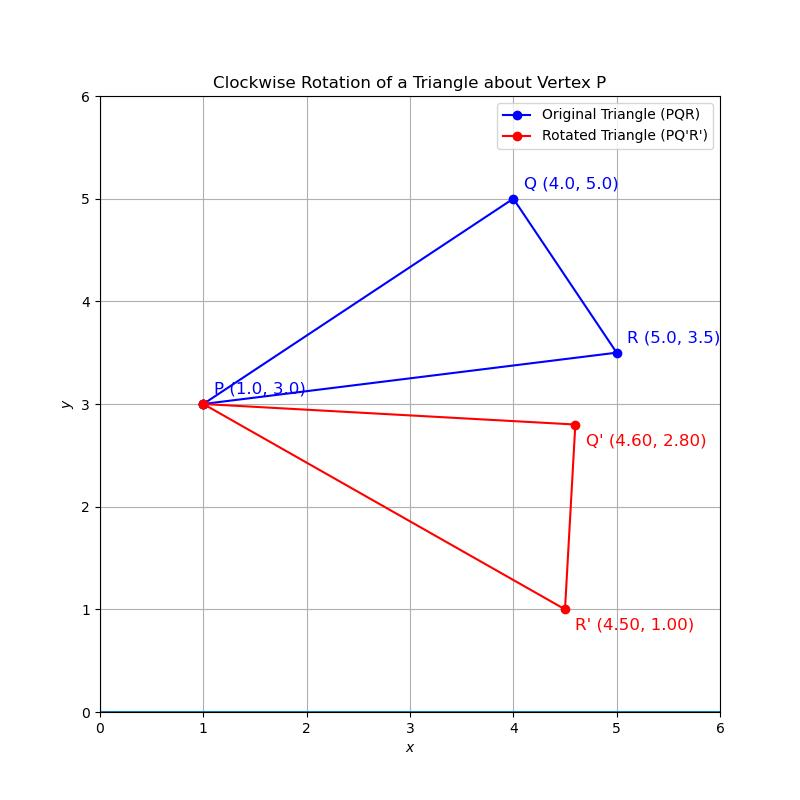
\includegraphics[width=\columnwidth]{figs/plot_c.jpg}
	\caption*{Plot}
	\label{fig:fig}
\end{figure}

\end{document}
